\section{Wide Column Stores}

Wide column stores were invented to provide more control over performance and in particular, in order to achieve high-throughput and low latency for objects ranging from a few bytes to about 10 MB.

\subsection{A sweet spot between object storage and relational database systems}

A wide column store has certain benefits over an object storage service.
\begin{itemize}
    \item A wide column store will be more tightly integrated with the parallel data processing systems. This is possible because the wide column store processes run on the same machines as the data processing processes, and it makes the entire system faster.
    \item Wide column stores have a richer logical model than the simple key-value model behind object storage.
    \item Wide column stores also handle very small values (bytes and kBs) well thanks to batch processing.
\end{itemize}
Note that a wide column store is not a relational database management system:
\begin{itemize}
    \item it does not have any data model for values, which are just arrays of bytes
    \item since it efficiently handles values up to 10 MB, the values can be nested data in various formats, which breaks the first normal form
    \item tables do not have a schema
    \item there is no language like SQL, instead the API is on a lower level and more akin to that of a key-value store
    \item tables can be very sparse, allowing for billions of rows and millions of columns at the same time; this is another reason why data stored in HBase is denormalized
\end{itemize}

\subsection{Logical Data Model}

\subsubsection{Rationale}
The data model of HBase is based on the realization that joins are expensive, and that they should be avoided or minimized on a cluster architecture. Joins can be avoided if they are pre-computed, that is, instead of storing the data as separate tables, we store, and work on, the joined table.

\subsubsection{Tables and row IDs}
From an abstract perspective HBase can be seen as an enhanced key- value store, in the sense that:
\begin{itemize}
    \item a key is compound and involves a row, a column and a version
    \item keys are sortable
    \item values can be larger (clobs, blobs), up to around 10 MB
\end{itemize}
On the logical level, the data is organized in a tabular fashion: as a collection of rows. Each row is identified with a row ID. Row IDs can be compared, and the rows are logically sorted by row ID.

\subsubsection{Column Families}
The other attributes, called columns, are split into so-called column families. This is a concept that does not exist in relational databases and that allows scaling the number of columns. Very intuitively, one can think of column families as the tables that one would have if the data were actually normalized and the joins had not been pre-computed.

\subsubsection{Column qualifiers}
Columns in HBase have a name (in addition to the column family) called column qualifier, however unlike traditional RDBMS, they do not have a particular type. In fact, it goes further than that. Not only are there no column types: even the column qualifiers are not specified as part of the schema of an HBase table: columns are created on the fly when data is inserted, and the rows need not have data in the same columns, which natively allows for sparsity.

\subsubsection{Versioning}
HBase generally supports versioning, in the sense that it keeps track of the past versions of the data. This is implemented by associating any value with a timestamp, also called version, at which it was created (or deleted). Users can also override timestamps with a value of their choice to have more control about versions.

\subsubsection{A multidimensional key-value store}
An HBase table is an enhanced key-value store where the key is four-dimensional. Indeed, in HBase, the key identifying the values in the cells consists of:
\begin{itemize}
    \item row ID
    \item column family
    \item column qualifier
    \item version
\end{itemize}

\subsection{Logical Queries}

\subsubsection{Get}
With a get command, it is possible to retrieve a row specifying a table and a row ID. Optionally, it is also possible to only request some but not all of the columns, or to request a specific version, or the latest k versions (where k can be chosen) within a time range (interval of versions).

\subsubsection{Put}
Wit a put command, it is possible to put a new value in a cell by specifying a table, row ID, column family and column qualifier. It is also possible to optionally specify the version. If none is specified, the current time is used as the version. HBase ofers a lockin gmechanism at the row level, meaning that different rows can be modified concurrently, but the cell in the same row cannot: only one user at a time can modify any given row.

\subsubsection{Scan}
With a scan command, it is possible to query a whole table or part of a table, as opposed to a single row. It is possible to restrict the scan to specific columns families or even columns. It is also possible to restrict the scan to an interval of rows. It is possible to run the scan at a specific version, or on a time range. Scans are fundamental for obtaining high throughput in parallel processing.

\subsubsection{Delete}
With a delete command, it is possible to delete a specific value with a table, row ID, column family and qualifier. Optionally, it is also possible to delete the value with a specific version, or all values with a version less or equal to a specific version.

\subsection{Physical architecture}

\subsubsection{Partitioning}
A table in HBase is physically partitioned in two ways: on the rows and on the columns. The rows are split in consecutive regions. Each region is identified by a lower and an upper row key, the lower row key being included and the upper row key excluded.
A partition is called a store and corresponds to the intersection of a region and of a column family.


\subsubsection{Network topology}
HBase has exactly the same centralized architecture as HDFS.

\begin{figure}[h]
    \centering
    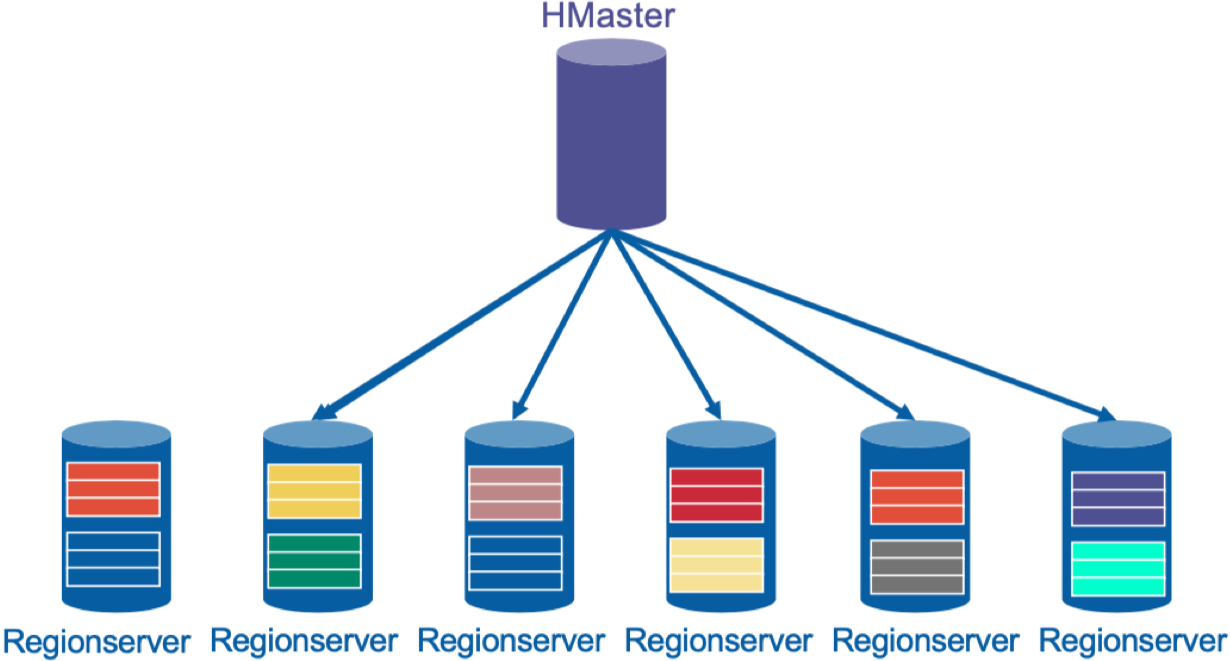
\includegraphics[width=0.7\textwidth]{Figures/HBaseNetworkTopology.jpeg}
    \caption{Network Topology of HBase.}\label{fig:HBNetTop}
\end{figure}

The HMaster and the RegionServers should be understood as pro- cesses running on the nodes, rather than the nodes themselves, even though it is common to use “HMaster” to designate the node on which the HMaster process runs, and “RegionServer” to designate a node on which a RegionServer process runs.

Remember, the namenode in HDFS does all the metalabel things. Creating directories, writing directories, deleting directories, etc. These are called DDL Operationd (Data Definition Language). The HMaster has other tasks than just that. It assigns regions to RegionServers. This means, for a given region (remember: interval of row IDs), all column families – each one within this region being a store – are handled by the same RegionServer.

There is no need to attribute the responsibility of a region to more than one RegionServer at a time because, as we will see soon, fault tolerance is already handled on the storage level by HDFS.

If a region grows too big, for example because of many writes in the same row ID interval, then the region will be automatically split by the responsible RegionServer. Note, however, that concentrated writes (“hot spots”) might be due to a poor choice of row IDs for the use case at hand. There are solution to this such as salting or using hashes in row ID prefixes.

If a RegionServer has too many regions compared to other Region-Servers, then the HMaster can reassign regions to other RegionServers.

Likewise, if a RegionServer fails, then the HMaster can reassign all its regions to other RegionServers.


\subsubsection{Physical Storage}
As we saw, the data is partitioned in stores, so we need to look at how each store is physically stored and persisted. The store is, physically, nothing less than an organized set of cells.

Each value in a cell is identified by a row ID (within the region handled by the store), a column family (the one handled by the store), a column qualifier (arbitrary) and a version (arbitrary). The version is often implicit as several versions of the same cell can co-exist with the latest one being current, but it is an important component in the identification of a value in a cell. This tuple of four values will be referred to as the key (of the value in the cell).

Each value in a cell is thus handled physically as a key-value pair where the key is a (row ID, column family, column qualifier, version) tuple.

All the cells within a store are eventually persisted on HDFS, in files that we will call HFiles. An HFile is, in fact, nothing else than a (boring) flat list of KeyVal- ues, one per version of a cell. What is important is that, in an HFile, all these KeyValues are sorted by key in increasing order, meaning, first sorted by row ID, then by column family (trivially unique for a given store), then by column qualifier, then by version (in decreasing order, recent to old). This means that all versions of a given cell that are in the same HFile are located together, and one of the values (within this HFile) is the latest.

HBase guarantees ACID on the row level (concurrent writes and reads are synchronizing with per-row locks). Clients therefore can access different rows at the same time, but two clients cannot access the same row simultaneously.

Of course, on the disk, a file is a sequence of 0s and 1s with no tabular structure, so that what in fact happens is that the KeyValues are stored sequentially. Now if we zoom in at the bit level, a KeyValue consists of four parts:
\begin{itemize}
    \item The length of the keys in bits (this length is encoded on a constant, known number of bits)
    \item The length of the value in bits (this length is encoded on a constant, known numbebr of bits)
    \item The actual key (of variable length)
    \item The actual value (of variable length)
\end{itemize}
The reason why we have the keylength and the valuelength at the beginning, is that the key and the value may hava variable lengths. Both, keylength and valuelength, are stored as 32 bits, thus 64 bits in total.

Zooming in even further, the key is itself made of the row ID, the column family, the column qualifier and the timestamp. We need also a row ID length and a column family length (similar to the key length and the value length). The timestamp has a fixed length (64 bits) and does not need additional input on its length. Finally the last byte (named “key type” for some reason) is mostly used as a deletion flag that indicates that the content of the cell, as of this version, was deleted. The reason why we don't need to specify the column qualifier length, is that we already know the key length, the row length and the column family length. Furthermore, the timestamp and the key type length are fixed. Thus, by simple subtraction, we obtain the column qualifier length.

\begin{figure}[h]
    \centering
    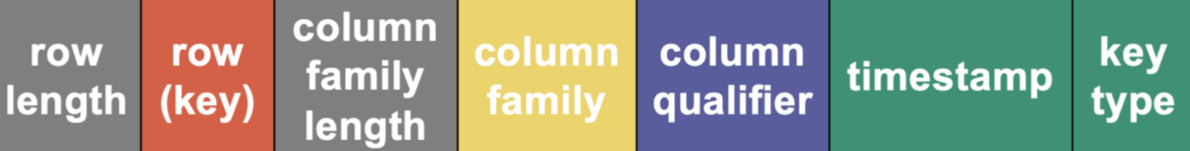
\includegraphics[width=0.7\textwidth]{Figures/KeyValueStructure.jpeg}
    \caption{Structure of a KeyValue}\label{fig:keyValStru}
\end{figure}

KeyValues, within an HFile, are organized in blocks. But to not confuse them with HDFS blocks, we will call them HBlocks. HBlocks have a size of 64 kB, but this size is variable: if the last KeyValue goes beyond this boundary, then the HBlock is simply longer and stops whenever the last KeyValue stops. The HFile then additionally contains an index of all blocks with their key boundaries. This separate index is loaded in memory prior to reading anything from the HFile. It can then be kept in memory for subsequent reads. Thanks to the index, it is possible to efficiently find out in which HBlock the KeyValues with a specific key (or within a specific key range) are to be read.

\begin{figure}[h]
    \centering
    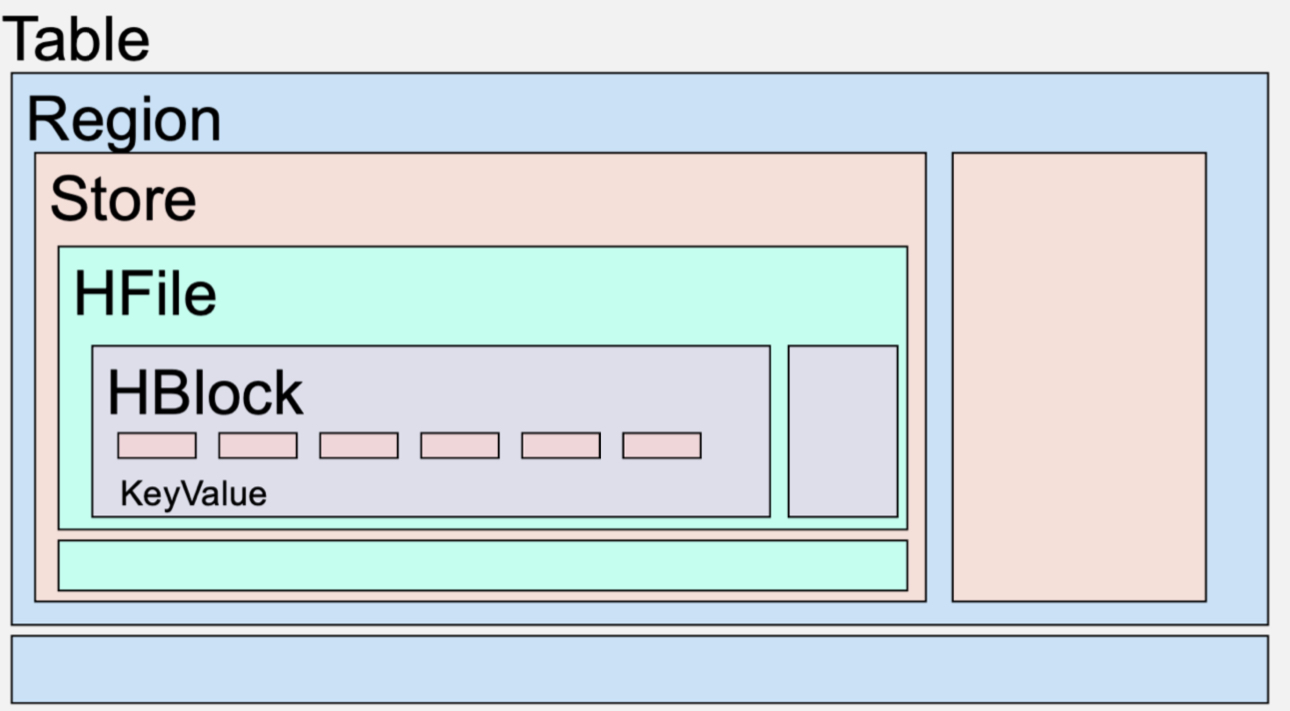
\includegraphics[width=0.7\textwidth]{Figures/SummaryPhysicalStorage.jpeg}
    \caption{Summary of the entire physical Storage hierarchy of KeyValues on HDFS.}\label{fig:SumPhysStor}
\end{figure}

There is one big problem. We can only write key-values in sorted order (append). How can we insert new values without having to rewrite the whole table?

\subsubsection{Log-structured merge trees}

Generally, “old” data is persisted to HDFS in HFiles, while “fresh” data is still in memory on the RegionServer node, and has not been persisted to HDFS yet. Thus, when accessing data, HBase needs to generally look every- where for cell values (i.e., physically, KeyValues) to potentially return: in every HFile, and in memory. As long as there is room in memory, freshly created KeyValues are added in memory. At some point, the memory becomes full (or some other limits are reached). When this happens, all the KeyValues need to be flushed to a brand new HFile. Upon flushing, all KeyValues are written sequentially to a new HFile in ascending key order, HBlock by HBlock, concurrently building the index structure. In fact, sorting is not done in the last minute when flushing. Rather, what happens is that when KeyValues are added to memory, they are added inside a data structure that maintains them in sorted order (such as tree maps) and then flushing is a linear traversal of the tree.

What happens if the machine crashes and we lose everything in memory? We have a so-called write-ahead-log for this. Before any fresh KeyValues are written to memory, they are written in sequential order (append) to an HDFS file called the HLog. There is one HLog per RegionServer. A full write-ahead-log also triggers a flush of all KeyValues in memory to a new HFile. If there is a problem and the memory is lost, the HLog can be retrieved from HDFS and “played back” in order to repopulate the memory and recreate the sorting tree structure.

Summary when to flush: Reaching max Memstore size in a store, reaching overall max Memstore size or reaching full write-ahead log.

After many flushes, the number of HFiles to read from grows and becomes impracticable. For this reason, there is an additional process called \textit{compaction} that takes several HFiles and outputs a single, merged HFile. Since the KeyValues within each HFile are already sorted, this can be done in linear time, as this is essentially the merge part of the merge-sort algorithm.

With flushing and compaction, we are starting to see some cycle of persistence. On a first level, the KeyValues in memory, on a second level, the KeyValues that have been flushed, on the third level, the KeyValues that have been flushed and compacted once, etc.

Compaction is not done arbitrarily but follows a regular, logarithmic pattern. Let us go through it. In a fresh HBase store, the memory becomes full at some point and a first HFile is output in a flush. Then the memory, which was emptied, becomes full again and a second HFile is output in a flush. This results in two HFiles of “standard size” that are immediately compacted to one HFile, twice as large. Then the memory, which was emptied, becomes full again and a new “standard-size” HFile is output in a flush. Then the memory, which was emptied, becomes full again and a second “standard-size” HFile is output in a flush. This results in two HFiles of “standard size” that are immediately compacted to one HFile, twice as large. This results in two HFiles of “double size” that are immediately compacted to one HFile, four times as large as the standard size. Then the memory, which was emptied, becomes full again and a new “standard-size” HFile is output in a flush. And so on...

\subsection{Additional design aspects}

\subsubsection{Bootstrapping lookups}
In order to know which RegionServer a client should communicate with to receive KeyValues corresponding to a specific region, there is a main, big lookup table that lists all regions of all tables together with the coor- dinates of the RegionServer in charge of this region as well as additional metadata (e.g. to support splitting regions, etc).
This big table is, in fact, also an HBase table, but it is special because this one fits on just one machine, known to everybody. Thus, the clients use this so-called meta table to know which RegionServers to communicate with.
To create, delete or update tables, clients communicate with the HMaster.

\subsubsection{Caching}
In order to improve latency, KeyValues that are normally persisted to HFiles (and thus no longer in memory) can be cached in a separate memory region, with the idea of keeping in the cache those KeyValues that are frequently accessed.
Caching is useless if we use batch processing, since in this case, we aggregate over the whole table anyway, or if we access the data randomly and uncontrolably.

\subsubsection{Bloom Filters}
HBase has a mechanism to avoid looking for KeyValues in every HFile. This mechanism is called a Bloom filter. It is basically a black box that can tell with absolute certainty that a certain key does not belong to an HFile, while it only predicts with good probability (albeit not certain) that it does belong to it. By maintaining Bloom filters for each HFile (or even each column), HBase can know with certainty that some HFiles need not be read when looking up certain keys.

\subsubsection{Data Locality and Short-Circuiting}
It is informative to think about the interaction between HBase and HDFS. In particular, recollect when we said that HDFS outputs the first replica of every block on the same (DataNode) machine as the client. Who is the client here? The RegionServer, which does co-habit with a DataNode. Now the pieces of the puzzle should start assembling in your mind: this means that when a RegionServer flushes KeyValues to a new HFile, a replica of each (HDFS) block of the HFile is written, by the DataNode process living on the same machine as the Region- Server process, to the local disk. This makes accessing the KeyValues in future reads by the RegionServer extremely efficient, because the RegionServer can read the data locally without communicating with the NameNode: this is known as short-circuiting in HDFS.

However, as time flies and the HDFS cluster lives its own life, some replicas might be moved to other DataNodes when rebalancing, making short-circuiting not (always) possible.
This, however, is not a problem, because with the log-structured merge tree mechanism, compactions happen regularly. And with every compaction, the replicas of the brand new HFile are again written on the local disk.

